\documentclass[12pt, a4paper]{article}

% !TeX root = ../main.tex
\usepackage{a4wide}

\usepackage[utf8]{inputenc}

%\usepackage[ngerman]{babel}
\usepackage[english]{babel}

\usepackage[T1]{fontenc}
\usepackage{palatino}

\usepackage{graphicx}
\usepackage{caption}
\usepackage{url}
\usepackage{tocloft}
\usepackage{acronym}

\usepackage{mathpazo}
\usepackage{amsmath}
\usepackage{amsfonts}
\usepackage{adjustbox}

%\usepackage{subcaption}

\usepackage{hhline}
\usepackage{amssymb}
\usepackage{floatflt}
\usepackage{setspace}
\usepackage{float}
\usepackage{color}
\usepackage{listings}
\usepackage{array}
\usepackage{scrhack}
\usepackage{xcolor}
\usepackage{wrapfig}
\usepackage{hyperref}
\usepackage{url}
\usepackage{lmodern}
\usepackage{multirow}
\usepackage{subfig}
\usepackage{cleveref}
\usepackage{lipsum}


% !TeX root = ../main.tex
%%%%%%%%%%%%%%%%%%%%%%%%%%%%%%%%%%%%%%%%%%%%%%%%%%%%%%%%%%%%%%%%%%%%%%%%
% Data about you and the Document%
%%%%%%%%%%%%%%%%%%%%%%%%%%%%%%%%%%%%%%%%%%%%%%%%%%%%%%%%%%%%%%%%%%%%%%%%

% % Main Title of Document:
\newcommand{\myMaintitle}{Untersuchung und Aufbau einer DevOps Development Umgebung}

% % Sub Title of DocInput:
\newcommand{\mySubtitle}{Developing holistic software solutions through integration of existing individual solutions.}

% % Ihr Name:
\newcommand{\myName}{Henrik Gerdes}

% % Matrikelnummer:
\newcommand{\myMatrikel}{MatNr: 969272}

% % Ihr Geburtsort:
\newcommand{\brith}{Osnabrück}

% % Ihr Geburtsort:
\newcommand{\place}{Osnabrück}

% % Ihr Abgabedatum:
\newcommand{\submission}{\today}

% % Ihr Abgabedatum:
\newcommand{\mycourse}{Exposé für den B.Sc.}

% % Name des Betreuers/Erstprüfenden:
\newcommand{\fistSupervisor}{Dennis Ziegenhagen}
\newcommand{\secSupervisor}{Achim Hendrix}

% % In welchem Semester befinden Sie sich?
\newcommand{\mySemester}{6. Semester}

\title{\myMaintitle}

\author{\myName}
% !TeX root = ../main.tex
% % Zeilenabstand im Haupttext auf anderthalb-zeilig setzen
%\linespread{1.25}\selectfont

% Line spacing
%\onehalfspacing{}

%Pfad für Grafiken
\graphicspath{{fig/}}

%Styleregeln
\widowpenalty10000 % Vermeidet einzelne Zeilen eines Absatzes zu Beginn einer Seite
\clubpenalty10000 % Vermeidet einzelne Zeilen eines Absatzes am Ende einer Seite
\addtocontents{toc}{\protect\sloppy}
\setcounter{tocdepth}{3}


% % \sloppy bewirkt, dass Latex beim Blocksatz nicht über den rechten Rand hinausschreibt.
% % und dafür größere Lücken in einer Zeile in Kauf nimmt
\sloppy

% % Setzt Dokumenteigenschaften für PDFs, wenn das Paket 'hyperref' geladen wurde.
\hypersetup{pdftitle=\myMaintitle,pdfauthor=\myName,bookmarksopen=true}

%Source for picture captions
\newcommand{\source}[1]{\caption*{Source: {#1}} }

\newcommand{\code}[1]{\texttt{#1}}

\newcommand{\myparagraph}[1]{\paragraph{#1}\mbox{}\\}

\newcommand{\RM}[1]{\MakeUppercase{\romannumeral{} #1{}}}

\newcommand{\HRule}{\rule{\linewidth}{0.5mm}} % Defines a new command for horizontal


\definecolor{dkgreen}{rgb}{0,0.6,0}
\definecolor{gray}{rgb}{0.5,0.5,0.5}
\definecolor{mauve}{rgb}{0.58,0,0.82}

\lstset{ %
  language=Java,                  % the language of the code
  basicstyle=\footnotesize,       % the size of the fonts that are used for the code
  numbers=left,                   % where to put the line-numbers
  numberstyle=\tiny\color{gray},  % the style that is used for the line-numbers
  stepnumber=1,                   % the step between two line-numbers. If it's 1, each line
                                  % will be numbered
  numbersep=5pt,                  % how far the line-numbers are from the code
  backgroundcolor=\color{white},  % choose the background color. You must add \usepackage{color}
  showspaces=false,               % show spaces adding particular underscores
  showstringspaces=false,         % underline spaces within strings
  showtabs=false,                 % show tabs within strings adding particular underscores
  frame=single,                   % adds a frame around the code
  rulecolor=\color{black},        % if not set, the frame-color may be changed on line-breaks within not-black text (e.g. commens (green here))
  tabsize=4,                      % sets default tabsize to 2 spaces
  captionpos=b,                   % sets the caption-position to bottom
  breaklines=true,                % sets automatic line breaking
  breakatwhitespace=false,        % sets if automatic breaks should only happen at whitespace
  title=\lstname,                 % show the filename of files included with \lstinputlisting;
                                  % also try caption instead of title
  keywordstyle=\color{blue},          % keyword style
  commentstyle=\color{dkgreen},       % comment style
  stringstyle=\color{mauve}         % string literal style
}

%%%%%%%%%%%%%%%%%%%%%%%%%%%%%%%%%%%%%%%%%%%%%%%%%%%%%%%%%%%%%%%%%%%%%%%%%%%%%%%%%%%%%%%%%
%Examples
%%%%%%%%%%%%%%%%%%%%%%%%%%%%%%%%%%%%%%%%%%%%%%%%%%%%%%%%%%%%%%%%%%%%%%%%%%%%%%%%%%%%%%%%%
% \pdfmarkupcomment[markup=Squiggly,color=green]{with pdfcomment}{move to the front}.
% \pdfmarkupcomment[markup=StrikeOut,color=red]{stupid}{replace stupid with funny}
% \pdfmarkupcomment[markup=Highlight,color=yellow]{Of course, you can highlight complete sentences.}{Highlight}
% \pdfcomment[icon=Note,color=blue]{insert graphic!}

% \pagestyle{plain}
\pagestyle{fancy}
\fancyhf{}
\fancyhfoffset[L]{1cm} % left extra length
\fancyhfoffset[R]{1cm} % right extra length
\rhead{\thepage}
\lhead{\nouppercase\leftmark}
\cfoot{\fancyplain{}{\thepage} }

\begin{document}

\pagenumbering{gobble}
% !TeX root = ../main.tex
%%%%%%%%%%%%%%%%%%%%%%%%%%%%%%%%%%%%%%%%%
% Academic Title Page
% LaTeX Template
% Version 2.0 (17/7/17)
%
% This template was downloaded from:
% http://www.LaTeXTemplates.com
%
% Original author:
% WikiBooks (LaTeX - Title Creation) with modifications by:
% Vel (vel@latextemplates.com)
%
% License:
% CC BY-NC-SA 3.0 (http://creativecommons.org/licenses/by-nc-sa/3.0/)
%
% Instructions for using this template:
% This title page is capable of being compiled as is. This is not useful for
% including it in another document. To do this, you have two options:
%
% 1) Copy/paste everything between \begin{document} and \end{document}
% starting at \begin{titlepage} and paste this into another LaTeX file where you
% want your title page.
% OR
% 2) Remove everything outside the \begin{titlepage} and \end{titlepage}, rename
% this file and move it to the same directory as the LaTeX file you wish to add it to.
% Then add \input{./<new filename>.tex} to your LaTeX file where you want your
% title page.
%
%%%%%%%%%%%%%%%%%%%%%%%%%%%%%%%%%%%%%%%%%

%----------------------------------------------------------------------------------------
%	TITLE PAGE
%----------------------------------------------------------------------------------------
%Titelseite
\begin{titlepage}
	\centering
	\thispagestyle{empty}
	\begin{center}
	
\includegraphics[width=0.9\textwidth]{uos.pdf}
	\end{center}
	\LARGE{\textsc{Institut für Informatik}}
	\vfill
	\textsc{\Large{\emph{\mycourse}}}\\[0.5cm]
	\HRule\\[0.4cm]
	\vspace{8mm}
	\huge{\textbf{{\fontfamily{ppl}\selectfont
	\myMaintitle}}}\\
	\HRule\\[0.4cm]
	\vspace{9mm}

	\begin{minipage}{0.4\textwidth}
		\begin{flushleft}
			\large
			\textit{Author}\\
			\textsc{\myName}\\ % Your name
			\textsc{\myMatrikel} % Your name
		\end{flushleft}
	\end{minipage}
	~
	\begin{minipage}{0.4\textwidth}
		\begin{flushright}
			\large
			\textit{Supervisor}\\
			\textsc{\fistSupervisor}\\ % Supervisor's name
			\textsc{\secSupervisor} % Supervisor's name
		\end{flushright}
	\end{minipage}

	\vspace{5cm}
	\large{\today}
	\vfill
	\end{titlepage}
	\newpage

% For printing add this
\newpage\null\thispagestyle{empty}\newpage

% Title & Abstract
\maketitle
\begin{abstract}
    \textbf{English:} \lipsum[20]
\end{abstract}
\begin{abstract}
    \textbf{German:} \lipsum[20]
\end{abstract}
\newpage

% Table of Contents
\tableofcontents
\newpage

% Normal page numbering
\newcounter{lastroman}
\setcounter{lastroman}{\value{page}}
\pagenumbering{arabic}

% Line spacing
% \onehalfspacing{}

\section{Introduction}\label{sec::intro}
Digital solutions are becoming more and more popular since the beginning of Industry 4.0 as a result of the ever-increasing possibilities and availability of technology. Due to the COVID-19 pandemic with new working and learning approaches, the need for digital business solution is bigger than ever before. To provide fast and suitable software solutions developers need adequate development setups, also called development environments. This thesis analysis modern agile software development environments point out potential problems and purposes a virtualized software development solution.\newline
This section provides an overview about this thesis. It will briefly describe the fundamental core question of this thesis, point out its relevance and presents a possible solution approach. Subsequently, a clear delineation is then given as to what is and is not covered in this thesis. The last section of the introduction gives a structural overview of how the thesis is structured and how it will approach the given problem.
    \subsection{Structural Overview}
    This section gives an initial overview and delineation to this thesis. Following this section, there is a description of the main topic of this work and the goal that should be achieved. Section \ref{sec::backgrund} provides overall background information, which are recommended for further understanding. Common and modern development methodologies are described in section \ref{ssec::devops}, followed by Microservice and container basics in section \ref{ssec::microservices} and \acl{CI} tools in \ref{ssec::ci_cd}. In section \ref{sec::problem} will be a detailed analysis of current development setups and the problems encountered in these setups. The problems are illustrated with examples and their consequences for the development process, the overall project and its quality, which is emblematic of user satisfaction, are presented. Section \ref{sec::solution_concept} proposes a conceptual solution, defines its usability and workings while also providing conditions and limitations for such a solution. This solution concept is applied in section \ref{sec::solution_code} by implementing it in a practical reference project. The implementation process is described and additional challenges and tricks for practical use are presented. Section \ref{sec::eval} discusses the proposed solution and shows its strengths and weaknesses. At the end, an outlook on future application areas and alternative solutions is given in section \ref{sec::outlook}, followed by the conclusion in section \ref{sec::conclusion}.

    \subsection{Problem Description}
    The rise of Agile development and Microservices was accelerated by the emergence of new technologies that changed the way \textit{where} and \textit{how} software is running. Applications could be distributed and scaled quickly through the Cloud which benefited customers favors for quick changes. Yet the actual coding setup has not changed significantly.\newline
    Requirements for development environments differ depending on the project type. The development process of (\acs{GUI}) applications for PC's and smartphones is quite different to web-services development. As the functionality of web services continues to grow, while being a cost-effective way to deliver across platforms products, this method is becoming increasingly popular. However, the operating system used for the development process often differs to the operating system used to run these applications in production. This can cause platform dependent errors. Managing language runtime versions between team members or different projects can also become a challenge, as these can lead to unexpected program behavior or result in library version conflicts. The usage of a microservice architecture, due to its easy scalability, adaptability and rapid development, brings further problems. Microservices require additional configuration effort and increases the difficulty level for whole system tests, also called end-to-end tests. The initial setup for new developers can get quiet complex, requires time and might even discourage developers in open source projects.\newline
    These characteristics add additional effort, can introduce new errors and slow down the development speed, resulting in higher cost and lower customer experience.

    \subsection{Scope of the Thesis}
    The range of different software development environments is large and differs significantly from each other depending on the project. As the development of web-based solutions is becoming more and more popular, priority is given only to these types of projects. Native application development for PCs and smartphones, as well as the development of embedded systems and other hardware-related solutions are not covered in this thesis.\newline
    In particular, the solution concept shown is not a general solution that is a perfect fit for all projects and therefore is not generally transferable. It is intended only as a solution template that contains many tricks for dealing with the problems described in section \ref{sec::problem}.

    \subsection{Goal of the Theses}
    In the process of this work, the challenges and obstacles of modern software development environments are identified and presented. Based on these findings, a solution concept, for these challenges, is created based on virtualization technologies. The technologies used are explained, and the solution concept is applied to a reference project. Subsequently, the practicability of the solution approach is evaluated and classified. In principle, the goal of this thesis is to identify obstacles in current software development setups and to analyze the effectiveness of the proposed solution.\newpage

\section{Background Information about Agile, Container and Microservices}\label{sec::backgrund}
The following section provides some basic definitions and principles that are necessary for the further understanding of this paper and ensures a common level of knowledge of these topics.\newline
First of will be a formal definition of DevOps, a brief description of the emergence and its current state.
    \subsection{Modern Methodologies: Agile and DevOps}\label{ssec::devops}
    This section provides a formal definition of agile software development Paradigms and the DevOps methodology, explains their connection and points out the fundamental principles of a DevOps enabled culture. These principles and their workflows will be revisited in section~\ref{sec::solution_concept} as part of the proposed solution concept.

        \subsubsection{Agile Development}
        Agile, just like the \wordhighlight{V-Model}, \wordhighlight{Waterfall} and \wordhighlight{Prototyping} model, is a software development paradigm. It was proposed and popularized by the \wordhighlight{"Manifesto for Agile Software Development"}, written and published in 2001 by various authors~\cite{manifesto}. Rapid adoption to changes, continuous evolution of software and customer communication are the fundamentals of agile software development.\newline
        The four core principles are:

        \begin{itemize}[label=\(\star\)]
            \setlength\itemsep{0em}
            \item \textbf{Individuals and interactions} over processes and tools
            \item \textbf{Working software} over comprehensive documentation
            \item \textbf{Customer collaboration} over contract negotiation
            \item \textbf{Responding to change} over following a plan
        \end{itemize}

        \noindent Paradigms like Waterfall describe a comprehensive model with a detailed requirements analysis and architecture design phase. This results in a fixed and detailed sequential schedule for the implementation, testing and requirements fulfillment verification phase. Errors in the requirements analysis or changes in requirements can cause difficulties later phases of the project. Agile on the other handle only provides guidelines instead of a complete model. Changes are expected and the project realization is designed to be adaptable. Project phases such as implementation and testing run together and the entire \ac{SDLC} is kept shorter and more adaptive \cite{agile_practice}.\newline
        Agile provides a mindset for projects with uncertain or continuous changing requirements. Accordingly, the agile manifesto became the foundation of several software development mythologies and frameworks that extend these fundamental guidelines and provide additional workflows and tooling for the software creation process. Well known examples are methodologies such as \wordhighlight{SCRUM}, \wordhighlight{\ac*{XP}} and \wordhighlight{DevOps}.

        \subsubsection{DevOps Definition}
        DevOps is a set of practices in software development hat aims to increase costumer value and software quality by shortening the development life cycle through active collaboration and continuous delivery of improvements \cite{base_devops}, \cite{effective_devops}. The term \wordhighlight{DevOps} is a neologism from development (Dev) and operation (Ops). The combination of these terms is symbolic for the tighter collaboration between the development and operations team, which were previously strictly separated. Therefore, DevOps is considered more than just software development principles, it is called a mindset and company/development culture. Shorter development times and closer collaboration are goals of agile software development paradigm. DevOps builds upon the guidelines and goals of agile and offers additional workflows and tools for software development to increased user experience value \cite{azuredevops}, \cite{effective_devops}.

        \subsubsection{Principles of DevOps}\label{ssec::devops_princibles}
        DevOps builds upon the agile principles. It extends the \wordhighlight{\acl{XP}} approach by also applying its principles to the operations and infrastructure aspects of the application \cite{effective_devops}. The goal is to provide a structured and comprehensive process from coding up to application monitoring. This process is referred to as a workflow and the minimal steps in an exemplary workflow are shown in table~\ref{tab::devops_steps}~\cite{base_devops}.\newline

        \begin{table}[!h]
            \centering
            \begin{tabularx}{0.85\textwidth}{llX}
                \multicolumn{2}{l}{Step} & Description \\ \hline\hline
                1 & \textbf{Coding}& Code development \& review and source control.  \\
                2 & \textbf{Building}& \acs{CI} build and build status.  \\
                3 & \textbf{Testing}& \acs{CI} testing and testing feedback.  \\
                4 & \textbf{Packaging}& Bundle and package to a central registry.  \\
                5 & \textbf{Releasing}& Release management, approvals and automation.  \\
                6 & \textbf{Configuring}& Infrastructure configuration and management.  \\
                7 & \textbf{Monitoring}& Applications performance monitoring.  \\
            \end{tabularx}
            \caption{DevOps workflow steps.}
            \label{tab::devops_steps}
        \end{table}

        \noindent With such a workflow come tasks that are the core procedures in a DevOps environment. These tasks include configuration management, release management, \ac{CI}, \ac{CD}, \ac{IaC}, test automation and application performance monitoring~\cite{azuredevops}.\newline
        For the scope of this work, only solutions from configuration management, \ac{CI} and \ac{IaC} will be used to enable a homogeneous development environment. The configuration management is about versioning the applications runtime environment and how to set it up. It determines on how the application interacts with system and external interface services. Common configuration parameter are the compiler/interpreter version, resources and permission settings as well as domain-names or \acs{IP}-addreses of other (external) services \cite{base_devops}. A DevOps principled architecture has multiple deployment stages. A staging and live environment is considered minimal base of any such projects. Adding a local environment increases the overall amount configuration effort, requiring a reliable, efficient way to manage it. This is closely related to the \ac{IaC} principle, which describes the provisioning process of computing resources. Tools like Ansible, Puppet and Terraform can automatically create and set up new cloud \ac{VM}s specified in a playbook. Playbooks are structured policies written in a custom language which are also stored in version control \cite{ansible2020}, \cite{azuredevops}.\newline
        These files describe how the host operating system is configured. Changes on these files can be handled the same way as regular code, starting with a pull request, reviews, test and approval of the changes. The \acl{IaC} principle will later be used to properly handle the setup of development containers, next to the \acs{CI} tools wich are described in section \ref{ssec::ci_cd}.

    \subsection{Container and Microservice Concept}\label{ssec::microservices}
    The following section provides a basic understanding about the concepts of Microservices and what principles are used to enable these.

        \subsubsection{Fundamental Idea of Microservices}
        The fundamental idea of Microservices is to have small independently deployable software applications. Connections between these applications make it possible to provide a greater service with an extensive range of functions \cite{micro}. An exemplary structure of a microservice cluster is visualized in figure \ref{fig::micro}. It shows multiple Microservices that each expose one functionality to the outside world. Application end-points such as a \ac{UI} provide a broad function range by internally calling multiple Microservices. In the event of one application failure, only that specific functionality becomes unavailable, the remaining system keeps operational. Because of this architectural design feature is advised that, while working with data, each microservice has its own Database. This prevents having a central database becoming a single point of failure. Another core feature of Microservices in its scalability. If the load on one part of the service increases, new instances of that application can be deployed to balance to load across all instances. This concept requires a fast and reliable process to create new application instances.\newline
        The installation and setup process of new hardware can be a time-consuming task. To reduce the amount of time it takes to create new application instances, the software industry uses the concept of virtualization.

        \begin{figure}
            \centering
            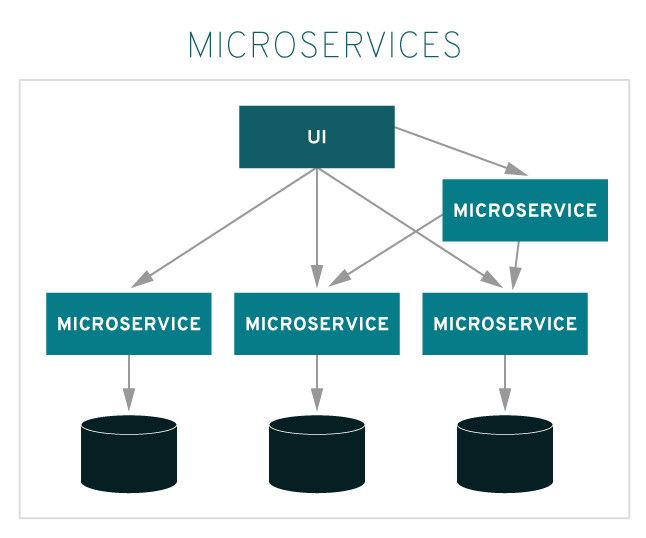
\includegraphics[width=0.5\textwidth]{monolithic-vs-microservices_altered.png}
            \caption{Structure of Microservices - [Altered], \\\textit{Source:~\cite{redhat_micro}}}\label{fig::micro}
        \end{figure}

        \subsubsection{Virtualization and Containerization}
        Virtualization is an abstraction layer. The physical hardware (called host) runs a hypervisor that allows the execution of (multiple) virtual machines (called guests) which act like a regular computer \cite{vmbasics}. This approach allows the usage of heterogeneous hardware without an impact on the guest operating systems thanks to the abstraction provided by the hypervisor. Without the need for specialized hardware and the dynamic allocation of resources, efficiency is also increased \cite{redhat_venv}. Additionally, virtual systems can be managed more easily because fundamentally they are just one big file on the host's storage device. They can be created on command, cloned and deleted without the configuration steps of a physical system. In the enterprise industry it is common to use this flexibility to start additional \ac{VM}s on high load. According to a study by the \ac{IDC} more than 80\% of data center workloads are virtualized \cite{virtualaddoption}. Virtualization also comes with the benefit of security. The majority of hypervisors strictly separate the host and the guest system. The guest system is not allowed to use the hosts resources and access its files unless it is explicitly configured to do so. Compromising a \ac{VM} does not affect the host or any other \ac{VM}s \cite{vmbasics}, \cite{redhat_venv}.\newline
        Full guest virtualization emulates a complete \ac{OS}, including the kernel, system libraries and even the majority of hardware devices. This abstraction comes with a performance penalty called overhead \cite{vmbasics}. A supposedly more lightweight approach of virtualization is called containerization. Studies by Ericsson Research, Nomadic Lab \cite{ieee_perfomance} and the Zhengzhou University \cite{zhengzhou_university} conclude in fact that container based solution provide better performance especially in disk \acs{I/O} and network \acs{I/O} bound scenarios. Containerization focuses on the isolation of one application process in a virtual runtime using control groups and namespace technologies \cite{cgroups}. Unlike \ac{VM}s, system and kernel functions are not virtualized and are passed through to the host machine. The result is a reduction of overhead and the ability to run additional application instances compared to \ac{VM}s with the same amount of compute resources. Figure \ref{fig::vm_docker} visualizes the differences between these approaches. The left side shows a traditional \ac{VM} based approach, on top of the host \ac{OS} runs a hypervisor which provides three full guest \acl{OS}s each with one application. Each gust is fully isolated and with its own kernel, \ac{OS} and runtime libraries. The container based solution only needs the host \ac{OS} and provides multiple application instances with shared libraries and runtimes in separated, isolated namespaces.\newline
        Apart from the performance benefits, the presumably main advantage of containers is their scalability~\cite{cintainer_scale}. Which makes them an adequate fit for Microservices. The most popular container based virtualization solutions are Docker, Podman and LXC.

        \begin{figure}
            \centering
            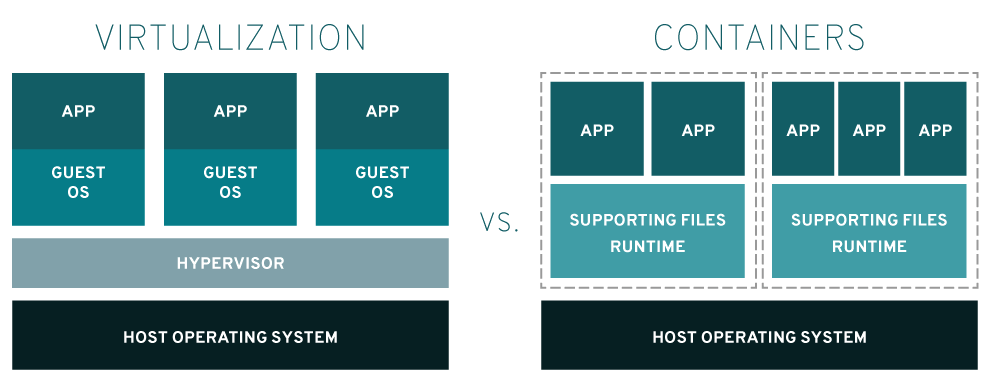
\includegraphics[width=0.9\textwidth]{docker-vm-redhat.png}
            \caption{\ac{VM}s compared to Containers, \\\textit{Source:~\cite{redhat_pic}}}\label{fig::vm_docker}
        \end{figure}

        \subsubsection{Usage of Containerization in Microservices}
        As described above, microservices are small applications that communicate with each other. To follow the principles for loose coupling between the applications the communication should be performed over a programming language independent protocol. Typical \acs{IP} network protocols used are \ac{REST}, WebSockets or GraphQL \cite{micro}. These loose coupled applications have the advantage that they can be development simultaneously from different teams as well as upgraded and replaced independently. As a result, applications can be developed much faster and more flexibly, following the principles of agile development \cite{micro}, \cite{redhat_micro}.\newline
        The usage of containers brings this speed and flexibility even further. Containers provide a consistent, isolated yet flexible runtime for applications \cite{micro_container}. Applications are packaged within known good runtimes. This reduces the setup time of the deployment and eliminate host specific errors. New application instances can be started without additional configuration. As a result of the successful concepts, tools like Docker Swarm and Kubernetes have been developed that can scale distributed applications in a managed dynamic, even automatic way.\newline
        \noindent Packaging and eventually even deploy the application introduces additional work for developers that was previously the task of the operations team. As already stated above, the developer and operations team are not separated in a DevOps culture. The new focus places value on team communication, flexibility and autonomy provided by the automation and support of as many steps as possible between the development and operation workflow \cite{effective_devops}. Eliminating manual tasks allows developers to focus on the actual application development. One of the main concepts in this process is the usage of \ac{CI} and \ac{CD} workflows.

    \subsection{Continuous Integration and Continuous Delivery Concepts}\label{ssec::ci_cd}
    \acl{CI} and \acl{CD} are two working concepts that are particularly well known in microservice architecture. Since every service provides only one part of the overall application functionality, it is uncertain what effects a change in one service has to other services and the wohle application.\newline
    \acl{CI} is a practice where new code is regularly integrated into the main code branch. Instead of having isolated functional branches that are worked on independently for months, changes flow back regularly to ensure it is free from conflicts and errors. Especially in interconnected services, it is important to ensure that a change in one service does not have an unintended effect on other services. \ac{CI} systems usually perform these integration tasks, as well as the associated tests automatically. In case of an error it becomes easier to identify the source error, due to these small and continuous integrations.\newline
    \acl{CD} on the other hand is a practice to bring these regular updates quickly and automatically into production. To ensure product quality, it is best to have multiple deployment environments, as described in section~\ref{ssec::devops_princibles}. Each new version is automatically deployed to a test or development environment where it undergoes automatic or manual testing. If the tests are successful, the version is promoted to the next deployment environment. In case of an error, the version is discontinued and the developers are notified about it. Only if all previous environments have not revealed any errors, the version will be transferred to production as a new release. Figure \ref{fig::cd} visualizes such a \ac{CD} pipeline. \newline
    Both \ac{CI} and \ac{CD} are practice to automate tasks that have previously been performed manually. Integration testing and packaging have both moved to a dedicated, autonomous system, giving developers and operators more time for other activities.
    % !TeX root = ../thesis_main.tex
\begin{figure}[]
    \centering
    \tikzstyle{block} = [rectangle, draw, fill=green!80!blue!70,
    text width=5em, text centered, rounded corners, minimum height=4em]
    \tikzstyle{line} = [draw, very thick, color=black!50, -latex']

    \begin{tikzpicture}[scale=2, node distance = 5cm, auto]
        % Place nodes
        \node [block] (init) {Code Check-in};
        \node [block, right of=init] (test) {\ac{CI} Pipeline \& Code-Test};
        \node [block, right of=test] (build) {Build \& Package Code};
        \node [block, below of=build, node distance=3.5cm] (d_test) {Deploy to Testing};
        \node [block, left of=d_test] (d_staging) {Deploy to Staging};
        \node [block, left of=d_staging] (d_live) {Deploy to Production};

        % Draw edges
        \path [line] (init) -- node {Triggers} (test);
        \path [line] (test) -- node {If successful} (build);
        \path [line] (build) -- node [left]{If successful} (d_test);
        \path [line] (d_test) -- node [above]{If successful} (d_staging);
        \path [line] (d_staging) -- node [above]{If successful} (d_live);
    \end{tikzpicture}
    \caption{\acl{CD} Workflow, \\\textit{Source: Modeled after~\cite{azuredevops}}}
    \label{fig::cd}
\end{figure}

\section{Analysis of the current State of Development Environments}\label{sec::problem}
The following section will display the current status of a typical \ac{DevEnv}, point out its problems and provides approaches for possible solutions.

\subsection{Current State of Developer Environments}
    Software development involves a broad variety of tasks. Depending on the project, tasks can range from pure web development, desktop or mobile application development, embedded system development or the pure maintenance of one of these variants. Each of these software development fields has its own workflows and requirements for the actual development setup. Even within these specialties, there are different requirements, depending on the scope, size, power and general capability demand for the project. Accordingly, development environments setups can differ greatly from one another.
    % Generalle Anforderung:
    % Fokus auf code nicht auf config.
    % Reproduzierbakeit
    % Kosten
    % Umgebung ist managbar

    % With the rise of cloud services the software development cycle accelerated. With services such as \ac{AWS}, Microsoft Azure and Google Cloud Computing it became possible to provision compute resources automatically and on demand. It changed the way \textit{where} and \textit{how} software is running.\newline
    % TODO
    \subsection{Common Issues in Modern Development Setups}
        \subsubsection{Additional Development Effort}
        \subsubsection{Issues Caused by Heterogeneous \acs{DevEnv}'s}
        \subsubsection{Operating System Specific Tools and Errors}
        \subsubsection{Dependencie Management}
        \subsubsection{Missing End-to-End Test Possibilities}
    \subsection{Propsed solution}

\section{Solution Concept of DevContainers}\label{sec::solution_concept}
    \subsection{Pre-requirements for DevContainers}
    \subsection{Description of a Conceptual Environment}
    \subsection{Available Tools and Resources}
    \subsection{Possible Implementations}
    \subsection{Strengths, Weaknesses and Limits}

\section{Exemplary Prototype Implementation}\label{sec::solution_code}
    \subsection{Current State and Goal}
    \subsection{Implementation Approach}
    \subsection{The Implementation Process}
    \subsection{Encountered Challenges and Limits}
    \subsection{Final state}

\section{Performance Evaluation and Analysis}\label{sec::eval}
    \subsection{Metrics and how to Evaluate}
    \subsection{Evaluation and Results}
    \subsection{Discussion of Evaluation}

\section{Future Potential and Outlook}\label{sec::outlook}
\section{Conclusion}\label{sec::conclusion}

\newpage
% Anhang
\lhead{Appendix}
\renewcommand{\thesubsection}{\Alph{subsection}}
\pagenumbering{Roman}
\setcounter{page}{\value{lastroman}}
\section*{Appendix}
\addcontentsline{toc}{section}{Appendix}

%Abkürzungsverzeichnis
% !TeX root = ../main.tex
\newcommand{\abbr}{Abbreviations}
\subsection{Abbreviations}
%\addcontentsline{toc}{subsection}{Abbreviations}

\begin{acronym}[1234567890]		%[längste Abkürzung]
\setlength{\itemsep}{-\parsep}	% sorgt dafür, dass das Verzeichnis kompakt dargestellt wird.

\acro{BLEST}[BLEST]{BLock ESTimation}
\acro{CWND}[CWND]{Congestion Window}
\acro{DAPS}[DAPS]{Delay-Aware Packet Scheduler}
\acro{ECF}[ECF]{Earliest Completion First}
\acro{HTTP}[HTTP]{Hypertext Transfer Protocol}
\acro{ISP}[ISP]{Internet Service Provider}
\acro{IETF}[IETF]{Internet Engineering Task Force}
\acro{LRF}[LRF]{Lowest-RTT-First}
\acro{MSS}[MSS]{Maximum Segment Size}
\acro{MPTCP}[MPTCP]{Multipath TCP}
\acro{MPTCPSW}[MPTCP\textsubscript{SW}]{MPTCP's send window}
\acro{OTIAS}[OTIAS]{Out-of-Order Transmission for In-Order Arrival Scheduler}
\acro{RR}[RR]{Round Robin}
\acro{RTT}[RTT]{Round Trip Time}
\acro{SCTP}[SCTP]{Stream Control Transmission Protocol}
\acro{sRTT}[sRTT]{Smoothed RTT}
\acro{STTF}[STTF]{Shortest Transfer Time First}
\acro{TCP}[TCP]{Transmission Control Protocol}
\acro{VoIP}[VoIP]{Voice over IP}
\end{acronym}
\newpage

%Code
% !TeX root = ../thesis_main.tex
\subsection*{Code for you}
\addcontentsline{toc}{subsection}{Code for you}
\begin{lstlisting}[frame=single, caption={DemoCode},label=code::sttf]
    int main(){
        int i;

        // Line comment.
        puts("Hello world!");

        for (i = 0; i < N; i++){
            puts("LaTeX is also great for programmers!");
        }

        return 0;
    }
\end{lstlisting}
\newpage
\listoffigures
\listoftables


%Bibliographie
\addcontentsline{toc}{section}{References}
\bibliographystyle{IEEEtranSA}
% \bibliographystyle{alpha}
\bibliography{bib/sources}
% !TeX root = ../main.tex
\section*{Declaration of Authorship}

\vspace{5cm}

~\\
I hereby declare that the paper submitted is my own unaided work. I assure that I wrote this paper without using any other means and sources than those specified. As well as the sources used literally or analogously taken from the sources identified as such.

\vspace{3cm}
\begin{flushright}

\rule{8cm}{0.2mm} \\
Signature (\myName)
\end{flushright}

\vspace{2cm}
\place, the \submission{}

\end{document}